\section{ATLAS work strategy}
\label{sec:ATLAS_work_strategy}

\subsection{The ATLAS Analyses and Publications}
\label{sec:The_ATLAS_Analyses_and_Publications}
ATLAS main objective is research to explain the nature of matter, physics  (from ancient Greek  phusikós), new phenomena, decay channels, discovery. To explain nature, it makes use of the gigantic hadron accelerator (LHC) and collide protons at the speed of light. With the cent er energy of 13 TeV provided by the accelerator, we explore matter, its interaction, its property and simulate small big bangs every second. Millions of particles collide in the accelerator and the ATLAS experiment is there to spy the evolution of these mini big bangs and try to make the most accurate interpretation. The results of this research complement our understanding of the nature of matter and the universe evolution itself. This information is recorded using mathematical tools, in the so called Standard Model and many other theoretical models.

To perform such a honourable search program, physicists need tools to analyse the data and compare them to the different models on the market. For this, ATLAS is organised in many Leading physics (PHY) and Combined performances (CP) groups and sub groups, under the coordination of main coordinators and conveners. These PHY and CP leading groups are, for example, Top quark (TOPQ), Standard Model (STDM), B quark (BPHY), Higgs (HIGG), Electron/Gamma (EGAM), Jet and Etmiss (JETM) etc. studies. Further studies on system detectors (SYS) or other activities like software (SOFT) and data preparation (DAPR) are also organized in leading groups and sub groups with main coordinators and conveners.

Once an analysis is finished or a detector performances is well studied, the physicist is asked to prepare a publication. In fundamental research, as this is the case with the research conducted at CERN, the communication to the public is not only compulsory but it is the exclusively way to demonstrate and show the results.

ATLAS considers three different types of publications: general publications based on data and the project related publications (PAPER), publications classified as notes (PUB notes), and conference proceedings (PROC) or notes (CONF Notes) on preliminary results aimed at conferences.
                    
All ATLAS analyses are discussed and presented in the relevant working groups (Physics, Combined performances, Systems and detectors, etc.). The Physics Coordinator, the working groups conveners and the Publication committee members are informed of all ongoing analyses and publications. They also appoint analysis contacts, contact editors, review experts. When the paper draft is ready, they set up an Editorial Board, set meetings dates to review the analysis and the goal of that analysis (CONF note, PAPER or PUB note).

\subsection{Author lists, acknowledgments and Proof Checker}
\label{sec:Authorlists_acknowledgments_and_ProofChecker}

Author lists and Acknowledgements are two of the main steps of a paper’s publication and both are handled and generated, using the FENCE framework, described in details in section~\ref{sec:The_FENCE_project}. Once the created author lists and acknowledgements are submitted to the journals, they come back to the ATLAS Physics Office for a final review before the publication. This review is mainly performed automatically using a PO tool: the proof checker.
                                                           
The author list is the inventory of qualified authors at a given date, which is also called the reference date. Every paper has a related list of qualified authors with a reference date which corresponds to the creation date of that list at the Paper Phase 1, just before the first circulation to the collaboration. Qualified authors are active physicists, still contributing to the maintenance and the operations of the collaboration. Some of them are retired people benefiting from their pre-data credits (worked before the data era), called signing-only authors. Between FENCE Phase 1 and Phase 2 (second circulation to the collaboration), some people may get exceptional authorship because of their involvement in the Analysis or the Paper. Therefore the author list is updated to include "exception" authors. The special cases are studied by the Authorship Committee and proposed for approval to the Spokesperson.
 
All this information is stored into the ATLAS database and managed by FENCE. Figure~\ref{fig:authorlist_generation} shows a full list of members (active and retired), their institutes and the related metadata that is needed to generate a full report of members and institutes.
\begin{figure}[ht!]
  \centering
  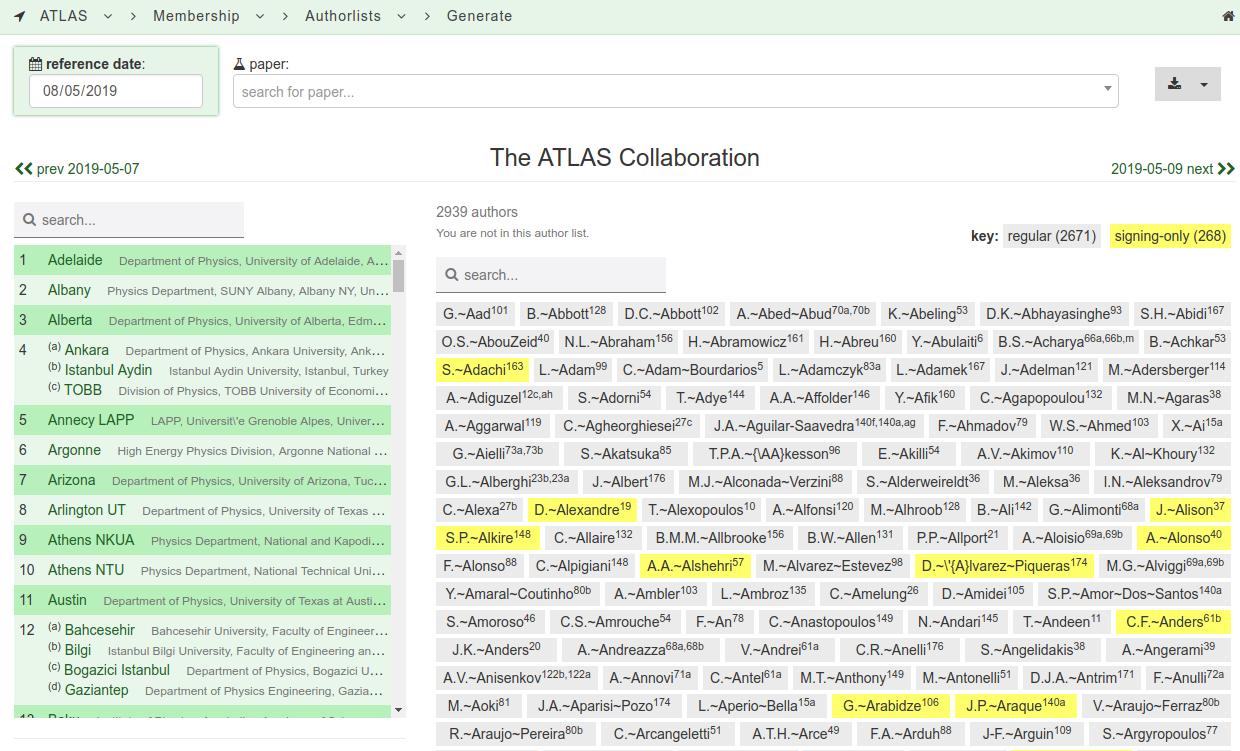
\includegraphics[width=0.9\textwidth]{figures/authorlist_generation.png}
  \caption{FENCE Author list generation interface.}
  \label{fig:authorlist_generation}
\end{figure}

The acknowledgements are a legal paragraph that the collaboration agrees to add in each Paper to thank Funding Agencies and Foundations financial support. They do not change very often but may include or suppress any other Funding Agency or Foundation at a given date. Therefore, an acknowledgement file is built for each paper at a specific date, which is called the reference date.
 
The proof checker is a tool provided mainly for the ATLAS PO members to compare the final publication (PDF file) of author lists and acknowledgement provided by the journal with ATLAS data (XML file). The main purpose of the proof checker is to identify inconsistencies between data provided to the journal and what the journal will produce as final output. A report of this comparison, one for every version of the proof, is available to the ATLAS PO members so they can check the results.
